\chapter{Operationen} \label{chap:operations}

    In diesem Kapitel werden wir uns den Zusammenhängen folgender Konzepte widmen:

    \begin{itemize}
        \item Operationen zwischen Graphen
        \item Operationen zwischen (oder auf) Matrizen von Graphen
        \item Spektrale Eigenschafte und Matrizen von Graphen
        \item Geometrische Eigenschaften von Graphen
    \end{itemize}

    \section{Unäre Operationen}

        \begin{definition} \label{def:operations_unary}

            \begin{enumerate}[
                label = \arabic*.,
                wide,
                labelindent = 0pt
            ]

                \item Sei $G$ ein ungerichteter (Multi-)Graph.
                Wir können den (Multi-)Graphen $G$ \textit{richten} und dessen \textit{gerichteten} Graphen $\vec G$ betrachten:
    
                \begin{align*}
                    V(\vec G) := V(G),
                    \quad
                    \text{und}
                    \quad
                    E(\vec G) := \bigcup_{\substack{\Bbraces{v, w} \in E(G) \\ v \neq w}} \Bbraces{(v, w), (w, v)} \cup \Bbraces{(v, v): \Bbraces{v, v} \in E(G)}.
                \end{align*}

                \item Sei $G$ ein gerichteter (Multi-)Graph.
                Wir können den (Multi-)Graphen $G$ \textit{entrichten} und dessen \textit{ungerichteten} Graphen $\bar G$ betrachten, mit Multi-Mengen als Kanten:
    
                \begin{align*}
                    V(\bar G) := V(G),
                    \quad
                    \text{und}
                    \quad
                    E(\bar G) := \Bbraces{\Bbraces{v, w}: (v, w) \in E(G)}.
                \end{align*}

                \item Sei $G$ ein Graph ohne ungerichtete Schleifen.
                Das \textit{Komplement} $G^\complement$ von $G$ sei definiert durch

                \begin{align*}
                    V(G^\complement) := V(G)
                    \quad
                    \text{und}
                    \quad
                    E(G^\complement)
                    :=
                    E(G)^\complement
                    =
                    \begin{cases}
                        V(G)^2 \setminus E(G),
                        & \text{wenn} ~ G ~ \text{gerichtet}, \\
                        \Bbraces{e \subseteq V(G): |e| = 2} \setminus E(G),
                        & \text{wenn} ~ G ~ \text{ungerichtet}.
                    \end{cases}
                \end{align*}

                \item Sei $G$ ein (Multi-)Graph.
                Wir definieren die \textit{Umkehrung} $G^\top$ von $G$ durch
    
                \begin{align*}
                    V(G^\top) := V(G)
                    \quad
                    \text{und}
                    \quad
                    E(G^\top)
                    :=
                    \begin{cases}
                        \Bbraces{(w, v): (v, w) \in E(G)},
                        & \text{wenn} ~ G ~ \text{gerichtet}, \\
                        E(G),
                        & \text{wenn} ~ G ~ \text{ungerichtet}.
                    \end{cases}
                \end{align*}

            \end{enumerate}    

        \end{definition}

        \begin{remark} \label{rem:operations_unary}

            Die Operationen in Definition \ref{def:operations_unary} sind vor allem dann wichtig, wenn man Ergebnisse von gerichteten auf ungerichtete Graphen (oder umgekehrt) übertragen will.
            Korollar \ref{cor:det} ist ein solches Beispiel.
            Dazu machen wir folgende Beobachtungen:

            \begin{enumerate}[
                label = \texttt{ad} \arabic*.,
                wide,
                labelindent = 0pt
            ]

                \item Seien $\mathbf A(G)$ und $\mathbf A(\vec G)$ die Adjazenz-Matrizen eines ungerichteten (Multi-)Graphen $G$ bzw. $\vec G$, zur selben Auflistung $(v_1, \dots, v_n)$ von $V(G)$.
                Die alten Kanten $\Bbraces{v, w}$ von $G$ tragen zur Adjazenz $\adj(v, w)$ sowie $\adj(w, v)$ bei, aber genauso tun das (gemeinsam) die beiden neuen Kanten $(v, w)$, $(w, v)$ von $\vec G$.
                Laut Konstruktion von $\vec G$ und der Definition der Adjazenz-Matrizen, ist

                \begin{align*}
                    \mathbf A(G) = \mathbf A(\vec G).
                \end{align*}

                Man beachte dabei, dass diese auf den Diagonalen deshalb übereinstimmen, weil ungerichtete Schleifen doppelt zur Adjazenz beitragen.

                Jedem vollständigen Teil-Graphen von $G$ mit $2$ Knoten, entspricht ein $2$-Zyklus in $\vec G$.
                Jedem Teil-$k$-Schaltkreis von $G$ entsprechen $2$ entgegengesetzte $k$-Zyklen in $\vec G$.
                Die folgende Abbildung \ref{fig:directing_sub_graphs} liefert ein paar Beispiele.

                \begin{figure}[h!]
                    \centering
                    \subfloat[vollständig mit $2$ Knoten $\mapsto$ $2$-Zyklus]
                    {
                        \begin{tikzpicture}

                            \begin{scope}[xshift = -1.5cm]

                                \filldraw (0,  1) circle (1pt) node (1_1_1) {};
                                \filldraw (0, -1) circle (1pt) node (1_1_2) {};

                                \draw [color = blue] (1_1_1) to (1_1_2);

                        \end{scope}

                        \draw node at (0, 0) {$\mapsto$};

                        \begin{scope}[xshift = 1.5cm]

                                \filldraw (0,  1) circle (1pt) node (1_2_1) {};
                                \filldraw (0, -1) circle (1pt) node (1_2_2) {};

                                \draw [->, color = blue] (1_2_1) to [bend right = 40] (1_2_2);
                                \draw [->, color = blue] (1_2_2) to [bend right = 40] (1_2_1);

                        \end{scope}

                        \end{tikzpicture}
                    }
                    \hspace*{2cm}
                    \subfloat[$1$-Schaltkreis $\mapsto$ zwei $1$-Zyklen]
                    {
                        \begin{tikzpicture}

                            \begin{scope}[xshift = -1.5cm]

                                \filldraw (0, 0) circle (1pt) node (2_1_1) {};

                                \draw [color = blue] (2_1_1) to [loop] ();

                        \end{scope}

                        \draw node at (0, 0) {$\mapsto$};

                        \begin{scope}[xshift = 1.5cm]

                            \filldraw (0, 0) circle (1pt) node (2_2_1) {};

                            \draw [->, color = red,   rotate =  90] (2_2_1) to [loop] ();
                            \draw [->, color = green, rotate = -90] (2_2_1) to [loop] ();

                        \end{scope}

                        \end{tikzpicture}
                    } \\
                    \subfloat[$2$-Schaltkreis $\mapsto$ zwei $2$-Zyklen]
                    {
                        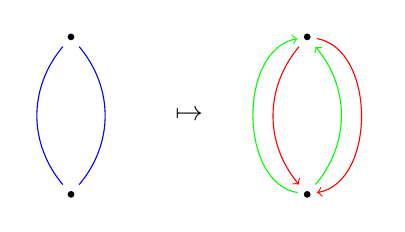
\begin{tikzpicture}

                            \begin{scope}[xshift = -1.5cm]

                                \filldraw (0,  1) circle (1pt) node (3_1_1) {};
                                \filldraw (0, -1) circle (1pt) node (3_1_2) {};

                                \draw [color = blue] (3_1_1) to [bend right = 40] (3_1_2);
                                \draw [color = blue] (3_1_2) to [bend right = 40] (3_1_1);

                        \end{scope}

                        \draw node at (0, 0) {$\mapsto$};

                        \begin{scope}[xshift = 1.5cm]

                                \filldraw (0,  1) circle (1pt) node (3_2_1) {};
                                \filldraw (0, -1) circle (1pt) node (3_2_2) {};

                                \draw [->, color = red]   (3_2_1) to [bend right = 40] (3_2_2);
                                \draw [->, color = green] (3_2_2) to [bend left  = 80] (3_2_1);

                                \draw [->, color = green] (3_2_2) to [bend right = 40] (3_2_1);
                                \draw [->, color = red]   (3_2_1) to [bend left  = 80] (3_2_2);

                        \end{scope}

                        \end{tikzpicture}
                    }
                    \hspace*{2cm}
                    \subfloat[$4$-Schaltkreis $\mapsto$ zwei $4$-Zyklen]
                    {
                        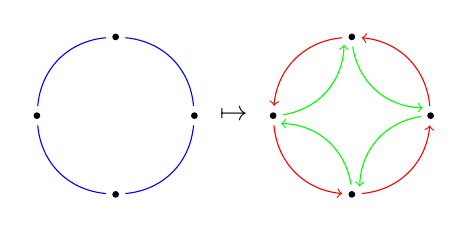
\begin{tikzpicture}

                            \begin{scope}[xshift = -1.5cm]

                                \filldraw (0, 1)  circle (1pt) node (4_1_1) {};
                                \filldraw (-1, 0) circle (1pt) node (4_1_2) {};
                                \filldraw (0, -1) circle (1pt) node (4_1_3) {};
                                \filldraw (1, 0)  circle (1pt) node (4_1_4) {};

                                \draw [color = blue] (4_1_1) to [bend right = 40] (4_1_2);
                                \draw [color = blue] (4_1_2) to [bend right = 40] (4_1_3);
                                \draw [color = blue] (4_1_3) to [bend right = 40] (4_1_4);
                                \draw [color = blue] (4_1_4) to [bend right = 40] (4_1_1);

                        \end{scope}

                        \draw node at (0, 0) {$\mapsto$};

                        \begin{scope}[xshift = 1.5cm]

                                \filldraw (0, 1)  circle (1pt) node (4_1_1) {};
                                \filldraw (-1, 0) circle (1pt) node (4_1_2) {};
                                \filldraw (0, -1) circle (1pt) node (4_1_3) {};
                                \filldraw (1, 0)  circle (1pt) node (4_1_4) {};

                                \draw [->, color = red]   (4_1_1) to [bend right = 40] (4_1_2);
                                \draw [->, color = green] (4_1_2) to [bend right = 40] ([shift = ({-0.1cm, -0.1cm})] 4_1_1);

                                \draw [->, color = red]   (4_1_2) to [bend right = 40] (4_1_3);
                                \draw [->, color = green] (4_1_3) to [bend right = 40] ([shift = ({0.1cm, -0.1cm})] 4_1_2);

                                \draw [->, color = red]   (4_1_3) to [bend right = 40] (4_1_4);
                                \draw [->, color = green] (4_1_4) to [bend right = 40] ([shift = ({0.1cm, 0.1cm})] 4_1_3);

                                \draw [->, color = red]   (4_1_4) to [bend right = 40] (4_1_1);
                                \draw [->, color = green] (4_1_1) to [bend right = 40] ([shift = ({-0.1cm, 0.1cm})] 4_1_4);

                        \end{scope}

                        \end{tikzpicture}
                    }
                    \caption
                    {
                        Durch das richten von $G$ entstehen aus den blauen Teil-Graphen links die blauen bzw. rot-grünen Teilgraphen rechts.
                        Die roten Zyklen verlaufen, wie gesagt, in die entgegengesetzte Richtung der grünen.
                    }
                    \label{fig:directing_sub_graphs}
                \end{figure}

                \item Seien nun $\mathbf A(G)$ und $\mathbf A(\bar G)$ die Adjazenz-Matrizen eines gerichteten (Multi-)Graphen $G$ bzw. $\bar G$, zur selben Auflistung $(v_1, \dots, v_n)$ von $V(G)$.
                Dadurch, dass die Richtung der Kanten $(v, w)$ bei $G \mapsto \bar G$ verloren geht, tragen diese nun nicht nur zur Adjazenz $\adj(v, w)$, sondern auch zu $\adj(w, v)$ bei.
                Das \enquote{spiegelt} sich in der Adjazenz-Matrix wieder, nämlich entlang der Diagonale.
                Man erhält
                
                \begin{align*}
                    \mathbf A(\bar G) = \mathbf A(G) + \mathbf A(G)^\top.
                \end{align*}

                Es sei abermals daran erinnert, dass das Summieren der Diagonalen zweckgemäß ist, da ungerichtete Schleifen doppelt zur Adjazenz beitragen.

                \item Seien $\mathbf A(G), \mathbf A(G^\complement) \in \Bbraces{0, 1}^{n \times n}$ die Adjazenz-Matrizen eines Graphen $G$ ohne ungerichtete Schleifen bzw. $G^\complement$, zur selben Auflistung $(v_1, \dots, v_n)$ von $V$.
                Für $i, j = 1, \dots, n$, sind $v_i, v_j$ genau dann adjazent in $G$, wenn $(v_i, v_j) \in E(G)$.
                Das gilt wiederum genau dann, wenn $(v_i, v_j) \not \in E(G^\complement)$.
                Daher gilt

                \begin{align*}
                    \mathbf A(G^\complement) = \mathbf J - \mathbf I - \mathbf A(G).
                \end{align*}

                \item Seien $\mathbf A(G)$ und $\mathbf A(G^\top)$ die Adjazenz-Matrizen eines (Multi-)Graphen $G$ bzw. $G^\top$, zur selben Auflistung $(v_1, \dots, v_n)$ von $V(G)$.
                Für $v, w \in V(G)$ gilt $(v, w) \in E(G)$ genau dann, wenn $(w, v) \in E(G^\top)$.
                Analoges gilt offenbar für die ungerichtete Kanten.
                Daher gilt

                \begin{align*}
                    \mathbf A(G^\top) = \mathbf A(G)^\top.
                \end{align*}

            \end{enumerate}

        \end{remark}

        \section{Geometrische Eigenschaften der Adjazenz-Matrix}

        \subsection{Die Determinante}

            \begin{theorem} \label{thm:det}

                Sei $G = (V, E)$ ein gerichteter (Multi-)Graph mit der Adjazenz-Matrix $\mathbf A = (a_{i,j})_{i,j=1}^n$ zur Auflistung $(v_1, \dots, v_n)$ von $V$.
                Dann gilt

                \begin{align} \label{eq:det_directed}
                    \det \mathbf A
                    =
                    \sum_{L \in \mathcal L_n}
                        (-1)^{p(L) + n}.
                \end{align}

            \end{theorem}

            \begin{proof}

                Wir zeigen die Aussagen zunächst für gerichtete Graphen (ohne Mehrfachkanten).

                Sei weiters

                \begin{align*}
                    S_n^\prime
                    :=
                    \Bbraces{\pi \in S_n: \Forall i = 1, \dots, n: a_{i, \pi(i)} > 0}.
                \end{align*}

                Laut Lemma \ref{lem:permutations} und \ref{lem:leibnitz} gilt

                \begin{align*}
                    \det \mathbf A
                    =
                    \sum_{\pi \in S_n}
                        \sgn \pi
                        \prod_{i=1}^n
                            a_{i, \pi(i)}
                    =
                    \sum_{\pi \in S_n^\prime}
                        (-1)^{p(\pi)}.
                \end{align*}

                Um weitere Gleichheit mit der rechten Seite von \ref{eq:det_directed} zu zeigen, konstruieren wir zunächst eine Bijektion zwischen $S_n^\prime$ und $\mathcal L_n$.

                \begin{enumerate}[label = \arabic*.]

                    \item Wir bauen für $\pi \in S_n$ einen Linear-Faktor $L \in \mathcal L_n$ von $G$.
                    Laut Lemma \ref{lem:permutations}, können wir $\pi$ in paarweise disjunkte (Permutations-)Zyklen $\pi_1, \dots, \pi_m \in S_n$ zerlegen, i.Z.

                    \begin{align*}
                        \pi = \pi_1 \circ \cdots \circ \pi_m,
                        \quad
                        \supp \pi = \dot \bigcup_{j=1}^m \supp \pi_j.
                    \end{align*}

                    Wir definieren entsprechende (Graphen-)Zyklen $C_1, \dots, C_m$ durch

                    \begin{multline*}
                        V(C_j) = \Bbraces{v_i: i \in \supp \pi_j}
                        \quad
                        \text{und}
                        \quad
                        E(C_j) = \Bbraces{(v_i, v_{\pi_j(i)}): i = 1, \dots, n}, \\
                        \text{für}
                        \quad
                        j = 1, \dots, m.
                    \end{multline*}

                    Offensichtlich sind das tatsächlich Zyklen.
                    Weil $i \mapsto v_i$ bijektiv ist, sind diese sogar paarweise disjunkt.
                    Wir definieren $L^\prime$ als deren direkte Summe:

                    \begin{align*}
                        L^\prime
                        :=
                        \bigoplus_{j=1}^n C_j.
                    \end{align*}

                    Momentan gilt noch

                    \begin{align} \label{eq:V_L_prime}
                        V(L^\prime)
                        =
                        \Bbraces{v_i: i \in \supp \pi}
                        \subseteq
                        V.
                    \end{align}

                    Weil ja $\pi \in S_n^\prime$ und damit die Koeffizienten von $\mathbf A$

                    \begin{align*}
                        a_{1, \pi(1)} = \cdots = a_{2, \pi(2)} = 1
                    \end{align*}

                    erfüllen, ist auch

                    \begin{align} \label{eq:E_L_prime}
                        E(L^\prime)
                        \subseteq
                        \Bbraces{(v_i, v_{\pi(i)}): i = 1, \dots, n}
                        \subseteq
                        E.
                    \end{align}

                    Wir wollen nun $L^\prime$ zu einem Linear-Faktor $L$ von $G$ erweitern.
                    Dazu, muss

                    \begin{align*}
                        V(L) = V.
                    \end{align*}

                    Außerdem müssen auch die Ausgangs- und Eingangs-Grade der Knoten aus $V \setminus V(L^\prime)$ gleich $1$ (und nicht $0$) sein.
                    Dazu fügen wir (gerichtete) Schleifen hinzu.
                    Laut \eqref{eq:V_L_prime}, ist

                    \begin{align*}
                        V \setminus V(L^\prime)
                        =
                        \Bbraces{v_i: i \not \in \supp \pi}.
                    \end{align*}

                    Laut \eqref{eq:E_L_prime}, ist daher

                    \begin{align*}
                        E(L)
                        :=
                        E(L^\prime) \cupdot \{ \underbrace{(v_i, v_i)}_{(v_i, v_{\pi(i)})}: 1, \dots, n = i \not \in \supp \pi \}
                        \subseteq
                        E.
                    \end{align*}

                    Seien nun

                    \begin{gather*}
                        V(C_j) = \Bbraces{v_{i_j}}
                        \quad
                        \text{und}
                        \quad
                        E(C_j) = \Bbraces{(v_{i_j}, v_{i_j})}, \\
                        \text{für}
                        \quad
                        j = m + 1, \dots, p(L)
                        \quad
                        \text{und}
                        \quad
                        \Bbraces{i_{m+1}, \dots, i_{p(L)}} = \Bbraces{1, \dots, n} \setminus \supp \pi,
                    \end{gather*}

                    so gilt

                    \begin{align*}
                        L = \bigoplus_{j=1}^{p(L)} C_j.
                    \end{align*}

                    \item Sei nun $L \in \mathcal L_n$ ein Linear-Faktor von $G$.
                    Sei $L := C_0$ die direkte Summe von (Graphen-)Zyklen $C_1, \dots, C_{p(L)}$:
                    Wir definieren entsprechende (Permutations-)Zyklen $\pi_1, \dots, \pi_{p(L)}$ sowie $\pi := \pi_0$ durch

                    \begin{multline*}
                        \pi_j(i)
                        :=
                        \begin{cases}
                            i^\prime, & \text{wenn} ~ \Exists i^\prime = 1, \dots, n: (v_i, v_{i^\prime}) \in E(C_j), \\
                            i,        & \text{sonst},
                        \end{cases} \\
                        \text{für}
                        \quad
                        i = 1, \dots, n,
                        \quad
                        \text{und}
                        \quad
                        j = 0, \dots, p(L).
                    \end{multline*}

                \end{enumerate}

                Abgesen von der Reigenfolgen der Zyklen, stimmen die Objekte der letzten beiden Schritte überein.
                Dies soll von der folgenden Abbildung \ref{fig:pi_vs_L} veranschaulicht werden.

                \begin{figure}[h!]
                    \centering
                    \begin{tikzpicture}[thick]

                        \begin{scope}

                            \filldraw (0, 2)  circle (1pt) node (1) {} node [above] {$v_i$};
                            \filldraw (2, 0)  circle (1pt) node (2) {} node [right] {$v_{i^\prime} = v_{\pi_j(i)}$};
                            \filldraw (0, -2) circle (1pt) node (3) {} node {};
                            \filldraw (-2, 0) circle (1pt) node (4) {} node {};

                            \draw [->] (1) to [bend left = 40] (2);
                            \draw [->] (2) to [bend left = 40] (3);
                            \draw [->] (3) to [bend left = 40] (4);
                            \draw [->] (4) to [bend left = 40] (1);

                            \node (label) at (0, 0) {$C_j \hateq \pi_j$};

                        \end{scope}

                        \begin{scope}[xshift = 3cm , yshift = 3cm]

                            \filldraw (0, 1)  circle (1pt) node (5) {};
                            \filldraw (0, -1) circle (1pt) node (6) {};

                            \draw [->] (5) to [bend left = 40] (6);
                            \draw [->] (6) to [bend left = 40] (5);

                        \end{scope}

                        \begin{scope}[xshift = 5cm , yshift = -3cm]

                            \filldraw (-1, 1) circle (1pt) node (7) {};
                            \filldraw (1, 1)  circle (1pt) node (8) {};
                            \filldraw (0, -1) circle (1pt) node (9) {};

                            \draw [->] (7) to [bend left = 40] (8);
                            \draw [->] (8) to [bend left = 40] (9);
                            \draw [->] (9) to [bend left = 40] (7);

                        \end{scope}

                        \node (dots) at (6, 0) {$\cdots$};

                    \end{tikzpicture}

                    \caption{Zusammenhang zwischen Linear-Faktor $L$ und Permutation $\pi$ sowie deren Zyklen}
                    \label{fig:pi_vs_L}
                \end{figure}

                Wir wollen nun auch noch zeigen, dass

                \begin{align} \label{eq:signs}
                    (-1)^{p(L) + n} = (-1)^{p(\pi)}.
                \end{align}

                Dabei ist $p(L)$ die Anzahl der Zusammenhangs-Komponenten (Zyklen) von $L$ und $p(\pi)$ die Anzahl der Fehlstände von $\pi$.
                Sei $j = 1, \dots, m$ und

                \begin{align*}
                    V(C_j) = \Bbraces{v_{i_{j, 1}}, \dots, v_{i_{j, |C_j|}}}
                    \quad
                    \text{und}
                    \quad
                    E(C_j) = \Bbraces{(v_{i_{j, 1}}, v_{i_{j, 2}}), \dots, (v_{i_{j, |C_j|}}, v_{i_{j, 1}})}.
                \end{align*}

                Wir können also $\pi_j$ als Produkt von $|C_j| - 1$ Transpositionen wie folgt schreiben:

                \begin{align*}
                    \pi_j
                    =
                    (i_{j, 1} \cdots i_{j, |C_j|})
                    =
                    (i_{j, 1} i_{j, 2}) \cdots (i_{j, |C_j|-1} i_{j, |C_j|}).
                \end{align*}

                Folgende Kongruenzen sind $\mod 2$ zu verstehen.
                Möge man nun $\pi$ ebenfalls als Produkt von $k$ Transpositionen schreiben, so gilt laut Lemma \ref{lem:permutations}, dass

                \begin{align} \label{eq:mod_1}
                    p(\pi)
                    \equiv
                    k
                    \equiv
                    \sum_{C \in \varepsilon(L)}
                        \underbrace
                        {
                            (|C| - 1)
                        }_{
                            \equiv 1
                        }
                    +
                    \sum_{C \in \omega(L)}
                        \underbrace
                        {
                            (|C| - 1)
                        }_{
                            \equiv 0
                        }
                    \equiv
                    e(L).
                \end{align}

                Weil $L$ direkte Summe der Zyklen $C_1, \dots, C_{p(L)}$ ist, gilt

                \begin{align} \label{eq:mod_2}
                    n
                    =
                    \sum_{C \in \varepsilon(L)} \underbrace{|C|}_{\equiv 0}
                    +
                    \sum_{C \in \omega(L)} \underbrace{|C|}_{\equiv 1}
                    \equiv
                    o(L).
                \end{align}

                Man beachte nun, dass $e(L) + o(L) = p(L)$.
                Setzt man \eqref{eq:mod_1} und \eqref{eq:mod_2} zusammen, so erhält man

                \begin{align*}
                    n + p(\pi) \equiv p(L).
                \end{align*}

                Daraus folgt offenbar \eqref{eq:signs}.

                Sei $G$ nun ein gerichteter Multi-Graph.
                Nun kann auch gelten, dass

                \begin{align*}
                    P_\pi
                    :=
                    \prod_{i=1}^n a_{i, \pi(i)}
                    >
                    1.
                \end{align*}

                Nachdem die Faktoren ja Koeffizienten von der Adjazenz-Matrix $\mathbf A$ sind, bedeutet das, dass wir bei der Wahl der Kanten $(v_i, v_{\pi(i)})$ genau $a_{i, \pi(i)}$ Möglichkeiten haben.
                Insgesamt können wir also, ausgegend von $\pi$, genau $P_\pi$ Linear-Fakteren $L \in \mathcal L_n$ (mit selbem $p(L)$) bauen.
                Umgekehrt, kommt man auf $\pi$ zurück durch genau $P_\pi$ viele Linear-Faktoren $L \in \mathcal L_n$ (mit selbem $p(L)$).

            \end{proof}

            Dieser Satz gilt auch für ungerichtete Multi-Graphen.

            \begin{corollary} \label{cor:det}

                Sei $G = (V, E)$ ein ungerichteter (Multi-)Graph mit der Adjazenz-Matrix $\mathbf A = (a_{i,j})_{i,j=1}^n$ zur Auflistung $(v_1, \dots, v_n)$ von $V$.
                Dann gilt

                \begin{align} \label{eq:det_undirected}
                    \det \mathbf A
                    =
                    \sum_{U \in \mathcal U_n}
                        (-1)^{p(U) + n} \cdot 2^{c(U)}.
                \end{align}

            \end{corollary}

            \begin{proof}

                Laut Bemerkung \ref{rem:operations_unary} und Satz \ref{thm:det}, gilt

                \begin{align*}
                    \det \mathbf A(G)
                    =
                    \det \mathbf A(\vec G)
                    =
                    \sum_{L \in \mathcal L_n(\vec G)}
                        (-1)^{p(L) + n}.
                \end{align*}

                Um zu zeigen, dass dies gleich der Rechten Seite von \eqref{eq:det_undirected} ist, bemühen wir abermals Bemerkung \ref{rem:operations_unary}, und zur Veranschaulichung eventuell die Abbildung \ref{fig:directing_sub_graphs}.
                Für jeden Teil-Schaltkreis von $U$ (insgesamt $c(U)$ viele) hat man zwei entstandene Zyklen zur Verfügung, um $L$ zu bilden.
                Daher entsprechen einer einfachen Figur $U \in \mathcal U_n(G)$ genau $2^{c(U)}$ viele Linear-Faktoren $L \in \mathcal L_n(\vec G)$ (mit selbem $p(L) = p(U)$).

            \end{proof}

            \begin{remark} \label{rem:induced_sub_graphs}

                Sei $\mathrm A$ Adjazenz-Matrix eines (Multi-)Graphen $G = (V, E)$ zur Aufzählung $(v_1, \dots, v_n)$ von $V$ ist.
                Sei weiters

                \begin{align*}
                    I = \Bbraces{i_1, \dots, i_m} \subseteq \Bbraces{1, \dots, n}
                \end{align*}

                Bezeichne $G_I$ den induzierten Teil-Graphen, der durch Löschen der Kanten $v_{i_1}, \dots, v_{i_m}$ aus $G$ entsteht.
                Dann ist $\mathrm A_I$ genau die entsprechende Adjazenz-Matrix von $G_I$.

            \end{remark}

        % Quelle: Spectra of Graphs - Theory an Application: On the number of walks, Seite 43
        \subsection{Die Anzahl der Pfade}

            Sei $G = (V, E)$ ein (Multi-)Graph.
            Wenn $G$ gerichtet ist oder keine Schleifen besitzt, so bezeichne $N_k(G; v, w)$, für $v, w \in V$, die Anzahl der Pfade in $G$ der Länge $k \in \N$ von $v$ nach $w$.
            Intuitiv kann man sich vorstellen, bei $v$ zu starten, dem Pfade Kante für Kante zu folgen, um dann bei $w$ anzugelangen.
            Was passiert aber, wenn $G$ ungerichtet ist und man dabei auf eine (ungerichtete) Schleife stößt und diese entlangmarschieren möchte?
            In welcher \enquote{Richtung} soll man sie passieren?

            \begin{enumerate}[label = \arabic*.]

                \item Aus intuitiver Sicht gibt es schließlich zwei Möglichkeiten.

                \item Aus mathematischer Sicht wäre dies unerheblich, weil $G$ ja ungerichtet ist, also keine \enquote{Richtung} existiert.
                Es gäbe also genau einen Pfad der Länge eins von dem Knoten in sich selbst, nämlich gerade den mit jener ungerichteten Schleife als Kante.

            \end{enumerate}

            Wir werden uns für die zweite Variante entscheiden.
            Man erinnere sich and die anfangs scheinbar willkürliche Konvention, dass ungerichtete Schleifen zum Grad und der Adjazenz eines Knoten zu sich selbst doppelt beitragen.
            Deswegen \enquote{scheinbar}, weil Bemerkung \ref{rem:operations_unary} darauf aufbaut (genauso deren Konsequenzen, z.B. in Form von Korollar \ref{cor:det}).
            Nur für dieses Teil-Teil-Kapitel wollen wir diese Konvention nicht einhalten.

            Man beachte allerdings, dass sich diese ungünstige Fallunterscheidung nur auf ungerichtete Graphen mit (ungerichteten) Schleifen bezieht.
            Wenn wir die Resultate hier einsetzen wollen und unsere Graphen keine ungerichteten Schleifen haben, so brauchen wir sie nicht zu beachten.

            \begin{theorem} \label{thm:number_of_paths}

                Sei $G = (V, E)$ ein (Multi-)Graph mit Adjazenz-Matrix $\mathbf A = (a_{i,j})_{i,j=1}^n$ zur Auflistung $(v_1, \dots, v_n)$ von $V$.
                Seien weiters $k \in \N$ und $\mathbf A^k = (a_{i,j}^{(k)})_{i,j=1}^n$.
                Dann ist die Anzahl der Pfade in $G$ der Länge $k$ von $v_i$ nach $v_j$, für $i, j = 1, \dots, n$, gleich

                \begin{align*}
                    N_k(v, w) = a_{i,j}^{(k)}.
                \end{align*}

            \end{theorem}

            \begin{proof}

                Wir verwenden Induktion nach $k \in \N$.

                Für $k = 0$ gilt $\mathbf A^k = \mathbf I$.
                Der einzige Pfad mit Länge $0$ ist das leere Wort $\varepsilon$.
                Wir vereinbaren, dass $\varepsilon$ immer von jedem Knoten zu sich selbst, nicht aber anderen Knoten in $G$, führt.

                Gelte nun die Aussage für $k \in \N$.
                Es gilt per definitionem $\mathbf A^{k+1} = \mathbf A^k \mathbf A$, und damit

                \begin{align} \label{eq:number_of_paths_induction}
                    a_{i,j}^{(k+1)}
                    =
                    \sum_{l=1}^n
                        a_{i,l}^{(k)}
                        a_{l,j}.
                \end{align}

                Um von $v_i$ nach $v_j$ zu gelangen, muss man vorhin bei $v_l$, für $l = 1, \dots, n$, gewesen sein und dann direkt nach $v_j$ gehen.
                Weil $a_{l, j} = \adj(v_l, v_j)$, gibt es für Letzteres genau so viele Möglichchkeiten.
                Laut Induktions-Hypothese, ist aber die Anzahl der Pfade in $G$ der Länge $k$ von $v_i$ nach $v_l$ gleich $a_{i,l}^{(k)}$.
                Daher gibt es $a_{i,l}^{(k)} a_{l,j}$ viele Pfade in $G$ der Länge $k+1$ von $v_i$ nach $v_j$, die durch $l$ verlaufen.
                Um letztere Bedingung zu eliminieren, muss man bloß über $l$ summieren.
                Dadurch erhält man aber genau die rechte Seite von \ref{eq:number_of_paths_induction}.

            \end{proof}

            \begin{corollary} \label{cor:number_of_paths_closed}

                Sei $G = (V, E)$ ein (Multi-)Graph mit einer Adjazenz-Matrix $\mathbf A$ und (gewöhnlichem) Spektrum $\sigma_P$.
                Dann ist die Anzahl der geschlossenen Pfade in $G$ der Länge $k \in \N$ gleich

                \begin{align*}
                    N_k^\prime(G)
                    =
                    \tr \mathbf A^k
                    =
                    \sum_{\lambda \in \sigma_P} \lambda^k.
                \end{align*}

                Insbesondere ist die Summe der Eigenwerte eines (Multi-)Graphen ohne Schleifen gleich $0$.

            \end{corollary}

            \begin{proof}

                Laut Satz \ref{thm:number_of_paths}, sind auf der Diagonale von $\mathbf A^k$ genau die Anzahlen der geschlossenen Pfade in $G$ der Länge $k$.
                $\tr A^k$ ist die Summe der Diagonale von $A^k$.
                Letztere Gleichheit gilt aufgrund von Lemma \ref{lem:trace} und \ref{thm:spectral_mapping_theorem}.
                Letzter Aussage gilt, weil alle Diagonal-Einträge einer Adjazenz-Matrix eines (Multi-)Graphen ohne Schleifen gleich $0$ sind.

            \end{proof}

            \begin{remark} \label{rem:number_of_paths_undirected}

                Sei $G = (V, E)$ ein ungerichteter (Multi-)Graph mit Adjazenz-Matrix $\mathbf A$ zur Auflistung $(v_1, \dots, v_n)$ von $V$.
                Weil $G$ ungerichtet ist, gilt für alle $i, j = 1, \dots, n$, dass $\adj(v_i, v_j) = \adj(v_j, v_i)$.
                $\mathbf A$ ist also symmetrisch.

                Laut \ref{thm:spectral_theorem}, hat $\mathbf A$ daher nur reelle Eigenwerte $\lambda_1 \leq \cdots \leq \lambda_n$ und es gibt eine orthogonale Matrix $\mathbf X = (x_{i,j})_{i,j=1}^n \in \operatorname O_n(\R)$, deren Spalten Eigenvektoren von $\lambda_1, \dots, \lambda_n$ sind und

                \begin{align*}
                    \mathbf \Lambda
                    :=
                    \diag(\lambda_1, \dots, \lambda_n)
                    =
                    \mathbf X^{-1} \mathbf A \mathbf X.
                \end{align*}

                Für $k \in \N$ gilt also

                \begin{align*}
                    (a_{i,j}^{(k)})_{i,j=1}^n
                    =
                    \mathbf A^k
                    =
                    (\mathbf X \mathbf \Lambda \mathbf X^\top)^k
                    =
                    \mathbf X \mathbf \Lambda^k \mathbf X^\top
                    =
                    \pbraces
                    {
                        \sum_{l=1}^n
                            x_{i,l} x_{j,l} \lambda_l^k
                    }_{i,j=1}^n
                \end{align*}

                Laut Satz \ref{thm:number_of_paths}, erhalten wir also

                \begin{align*}
                    N_k(G)
                    =
                    \sum_{i,j=1}^n
                        N_k(G; v_i, v_j)
                    =
                    \sum_{i,j=1}^n
                        a_{i, j}^{(k)}
                    =
                    \sum_{i,j=1}^n
                        \sum_{l=1}^n
                        x_{i,l} x_{j,l} \lambda_l^k
                    =
                    \sum_{l=1}^n
                        \pbraces
                        {
                            \sum_{i=1}^n
                                x_{i,l}
                        }^2
                        \lambda_l^k.
                \end{align*}

            \end{remark}

            \begin{proposition}

                Sei $G$ ein Graph ohne ungerichtete Schleifen mit einer Adjazenz-Matrix $\mathbf A$.
                Dann gilt für die \textit{generierende Funktion}

                \begin{multline*}
                    H(G; t)
                    :=
                    \sum_{k=0}^\infty N_k(G) t^k
                    =
                    \frac{1}{t}
                    \pbraces
                    {
                        (-1)^n
                        \frac
                        {
                            \chi_P
                            \pbraces
                            {
                                G^\complement;
                                -\frac{t+1}{t}
                            }
                        }{
                            \chi_P
                            \pbraces
                            {
                                G;
                                \frac{1}{t}
                            }
                        }
                        -
                        1
                    } \\
                    \text{für}
                    \quad
                    t \in \R \setminus \Bbraces{0}
                    \quad
                    \text{und}
                    \quad
                    \frac{1}{t} \not \in \sigma_P(G).
                \end{multline*}

            \end{proposition}

            \begin{proof}

                Es gilt $\mathbf I - t \mathbf A \in \operatorname{GL}_n(\R)$, weil

                \begin{align*}
                    0
                    \neq
                    t^n \chi_P \pbraces{G; \frac{1}{t}}
                    =
                    t^n \det \pbraces{\frac{1}{t} \mathbf I - \mathbf A}
                    =
                    \det(\mathbf I - t \mathbf A).
                \end{align*}

                Wir können also eine Neumann-Reihe (vgl. \cite[Kapitel 9.3]{Ana1&2}) und Lemma \ref{lem:cofactor_inverse} verwenden und erhalten

                \begin{align*}
                    \sum_{k=0}^\infty
                        t^k \mathbf A^k
                    =
                    (\mathbf I - t \mathbf A)^{-1}
                    =
                    \det(\mathbf I - t \mathbf A)^{-1} \cof(\mathbf I - t \mathbf A)
                \end{align*}

                Mit Satz \ref{thm:number_of_paths}, weil $\sum$ stetig ist und wegen der Distributivität, erhalten wir

                \begin{align} \label{eq:generating_function_eq_1}
                    H(G; t)
                    =
                    \sum_{k=0}^\infty
                        N_k(G) t^k
                    =
                    \sum_{k=0}^\infty
                        \sum \mathbf A^k
                            t^k
                    =
                    \sum
                        \sum_{k=0}^\infty
                            \mathbf A^k
                            t^k
                    =
                    \det(\mathbf I - t \mathbf A)^{-1} \sum \cof(\mathbf I - t \mathbf A).
                \end{align}

                Wir wenden Lemma \ref{lem:cofactor_sum} auf $\mathbf I - t \mathbf A$ und $t$ an und erhalten

                \begin{align*}
                    \det(\mathbf I - t \mathbf A + t \mathbf J)
                    =
                    \det(\mathbf I - t \mathbf A)
                    +
                    t \sum \cof(\mathbf I - t \mathbf A),
                \end{align*}

                also

                \begin{align} \label{eq:generating_function_eq_2}
                    \sum \cof(\mathbf I - t \mathbf A(G))
                    =
                    \frac{1}{t}
                    \pbraces
                    {
                        \det((t+1) \mathbf I + t \mathbf A(G^\complement))
                        -
                        \det(\mathbf I - t \mathbf A(G))
                    },
                \end{align}

                wobei $\mathbf A(G^\complement) = \mathbf J - \mathbf I - \mathbf A(G)$, laut Bemerkung \ref{rem:operations_unary}.
                Wenn wir nun \eqref{eq:generating_function_eq_2} in \eqref{eq:generating_function_eq_1} einsetzen und, so bekommen wir weiter

                \begin{align*}
                    =
                    \frac{1}{t}
                    \pbraces
                    {
                        (-1)^n
                        \frac
                        {
                            \det
                            \pbraces
                            {
                                -\frac{t+1}{t} \mathbf I - \mathbf A(G^\complement)
                            }
                        }{
                            \det
                            \pbraces
                            {
                                \frac{1}{t} \mathbf I - \mathbf A(G)
                            }
                        }
                        -
                        1
                    }
                    =
                    \frac{1}{t}
                    \pbraces
                    {
                        (-1)^n
                        \frac
                        {
                            \chi_P
                            \pbraces
                            {
                                G^\complement;
                                -\frac{t+1}{t}
                            }
                        }{
                            \chi_P
                            \pbraces
                            {
                                G;
                                \frac{1}{t}
                            }
                        }
                        -
                        1
                    }.
                \end{align*}

            \end{proof}
